\section{Motivation}\label{motivation}

\emph{This section is co-authored with Marissa Allen}

We set out to create a tool that would help people design 3D pop-up
cards. We were driven by the desire to create original kirigami designs
without a template. As we progressed in our project, we began to focus
on developing a tool that would provide a way to create pop-ups more
intuitively, without explicitly understanding how to create a valid
90-degree pop-up card. Our tool allows users to design, iterate, and
preview an original pop-up card before they even pick up a pair of
scissors.

\section{Technical Overview}\label{technical-overview}

\emph{This section is co-authored with Marissa Allen}

Our algorithmic simulation and validity detection is based on a tight
set of constraints to the pop-up card problem. We require the card to
have a central main valley fold --- from there we can determine the
orientation, as alternating folds fold in opposite orientations. The
card then folds 180 degrees; this implies parallelogram constraints
between all the edges in a sideways cross-section (with the exception of
v-fold features).

We capture touch input, translating touches into cuts and folds
depending on the geometry of the fold feature. We validate fold features
before they are added to the sketch, ensuring that the design can fold
in 3D. At this point, we also perform bezier path operations to modify
existing edges in the sketch based on the new design element. When a
fold feature is added to the sketch, we re-calculate planes (areas
enclosed by cuts and folds) by traversing a directed graph of edges in
the sketch. Based on these 2D planes, we create 3D planes, which are
oriented and translated based on their relationship to other planes in
the sketch. In 3D, we animate planes in response to user input. Each of
the planes is translated in relation to the plane oriented above the
fold and rotated in relation to the main driving joint.

Our approach constructs a tree representation of the planes based on
fold adjacency and uses this for determining the parent child
relationships in the simulated 3D view. We also use a tree-based
structure to store associations between logical geometric units.

\subsection{Development Process}\label{development-process}

We designed and developed the software interactively, frequently testing
prototypes with users. We used github to build Foldlings
collaboratively. Our workflow involved creating new code branches for
each feature, and reviewing the changes before merging back into the
master branch of the codebase. The full source for our software is
available at \url{http://github.com/harquail/foldlings/}.

\begin{figure}[htbp]
\centering
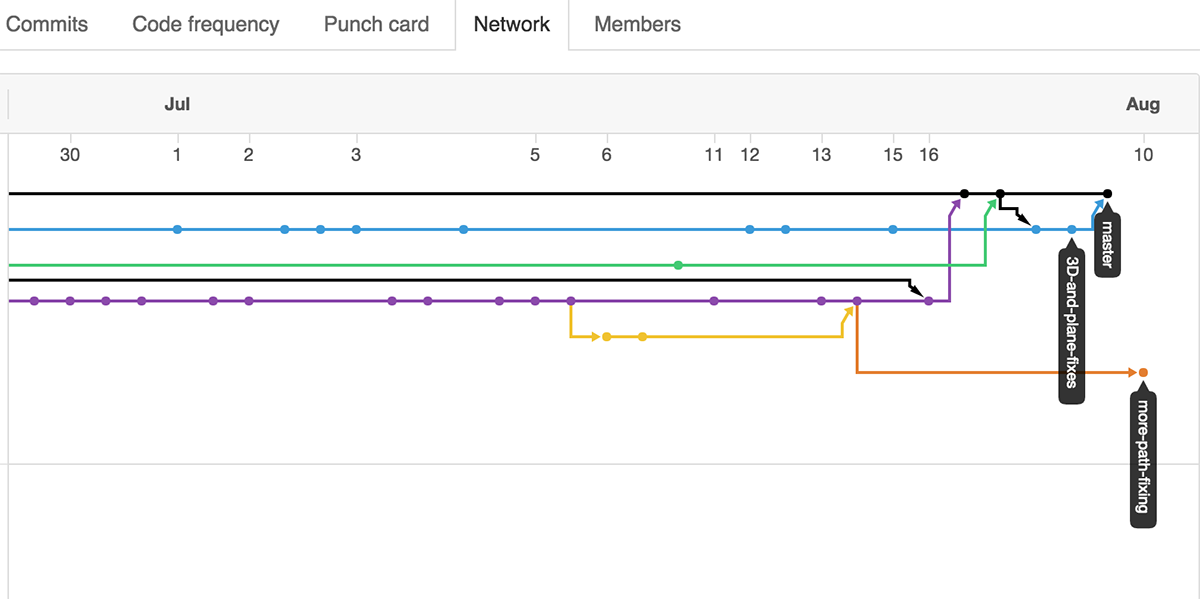
\includegraphics{figures/shared/02_Overview/gitflow.png}
\caption{Branches in our github.com repository.}
\end{figure}

\section{Pipeline Overview}\label{pipeline-overview}

\emph{This section is co-authored with Marissa Allen}

\begin{figure}[htbp]
\centering
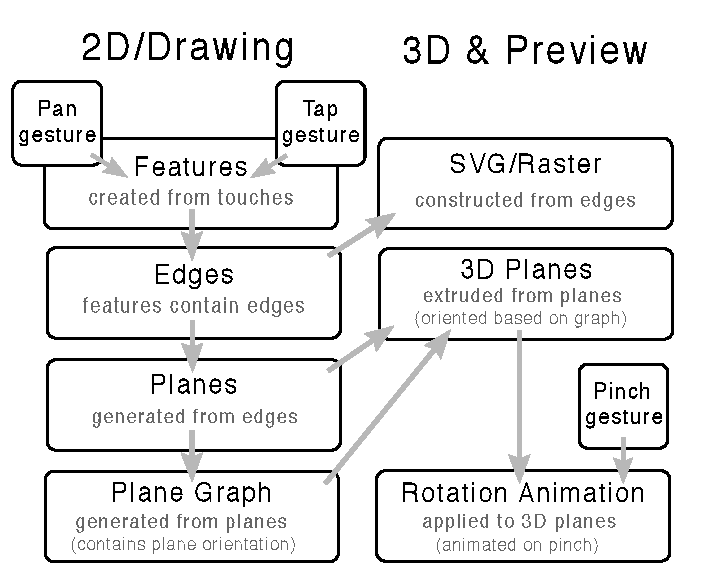
\includegraphics{figures/shared/02_Overview/pipeline.pdf}
\caption{Overview of data flow between 2D and 3D systems.}
\end{figure}

To begin, a user draws a design using the fold feature tools: box fold,
polygon, freeform and v-fold. These tools create a pattern of cuts and
folds, displaying an interactive preview of the design as the user
creates it. The cuts and folds created with these tools remain
associated with each other, and can be modified or deleted as a unit.

Each time a new shape is added to the design, it is evaluated for
validity: whether it can fold to 90 degrees and be parsed into
individual planes. The planes are then linked together in an acyclic
graph based on the planes' abutting top edges. This acyclic graph allows
us to shade planes based on orientation in 2D and simulate the design in
3D. Each feature can also be modified or deleted, by tapping on the
feature an selecting an entry from the list of available options.

This process continues until the user previews the design in 3D. The 3D
preview displays a simulation of how the design will fold, which can be
manipulated using a pinch gesture. The user is free to return to the 2D
drawing interface and continue editing his/her design or save the design
as either a raster file or SVG vector file. After this step, the user
can print and cut the raster file or open the SVG file on a laser cutter
or other cutting tool. We automatically save designs locally when
leaving the design workspace, so users can restore their work.
